\begin{center}
\textsc{Gauss} to \textsc{Olbers}.\quad Zeven, 4~July 1824.
\end{center}

\par\noindent\hspace*{\parindent}.\ .\ .\ .\ .\ .\quad The prospects for making further progress are extremely poor.
It will not be feasible to bypass Bremen as I had previously hoped, since
\par\smallskip\noindent\rule{.24\linewidth}{.4pt}\par\smallskip
{\footnotesize\noindent\hspace*{2.75em}[\textsuperscript{*}) See the letters to \textsc{Olbers} of 6~July 1824, p.~320, note, and of 1~March 1827, p.~378.]\par}
\par\smallskip\noindent{\footnotesize IX.}\hfill{\footnotesize47}\par
\clearpage
\noindent370\hfill{\small\textbf{CORRESPONDENCE WITH OLBERS.}}\par\medskip
\noindent Weierberg cannot be connected with Brüttendorf.
But there is \textls[120]{nothing at all} else satisfactory that can be connected with Brüttendorf to the northwest or north.
\textsc{Müller}'s reconnaissance from Bremervörde to Osterholz has yielded absolutely \textls[120]{no} result.
The only point would be near Wentel, but it would probably give an angle of only about \(12^{0}\) at Bremen, one of \(46^{0}\) at Brüttendorf, and one of \(122^{0}\) at Wentel, p[raeterpro]pter, and I have no idea yet whether the sacrifice I would make by using so poor a triangle
\par
\begin{center}
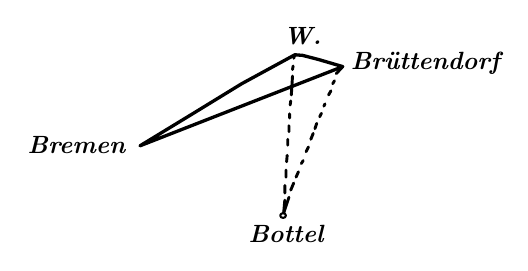
\begin{tikzpicture}[x=.0075cm,y=-.0075cm,line cap=round,line join=round]
\coordinate (Bremen) at (228,231);
\coordinate (Wentel) at (490,77);
\coordinate (Bruettendorf) at (571,97);
\coordinate (Bottel) at (470,349);
\draw[line width=1.2pt]
  (Bremen) -- (320,175) -- (400,126) -- (Wentel)
  -- (503,78) -- (530,85) -- (Bruettendorf) -- cycle;
\draw[line width=1.05pt]
  (Wentel) -- (488,83)
  (487,96) -- (486,102)
  (486,113) -- (484,145)
  (483,155) -- (482,162)
  (481,177) -- (481,184)
  (480,197) -- (480,207)
  (478,220) -- (478,230)
  (477,247) -- (476,258)
  (475,272) -- (475,284)
  (473,298) -- (473,311)
  (473,323) -- (471,345);
\draw[line width=1.05pt]
  (Bruettendorf) -- (560,109)
  (557,121) -- (554,126)
  (551,138) -- (547,145)
  (541,160) -- (539,164)
  (535,176) -- (532,182)
  (527,193) -- (524,202)
  (521,210) -- (517,220)
  (513,233) -- (509,241)
  (504,256) -- (501,261)
  (496,275) -- (492,284)
  (488,294) -- (483,306)
  (480,318) -- (471,345);
\draw[line width=.75pt,fill=white] (Bottel) ellipse [x radius=.36mm,y radius=.30mm];
\node[font=\small\bfseries\itshape,inner sep=0pt,anchor=east] at (204,229) {Bremen};
\node[font=\small\bfseries\itshape,inner sep=0pt,anchor=south] at (503,61) {W.};
\node[font=\small\bfseries\itshape,inner sep=0pt,anchor=west] at (584,92) {Brüttendorf};
\node[font=\small\bfseries\itshape,inner sep=0pt,anchor=north] at (475,365) {Bottel};
\end{tikzpicture}
\end{center}
\noindent (which would be somewhat improved if Wentel could also be connected with Bottel) would be offset by a reasonably good prospect northwest of Wentel.
In the end I may therefore still have to include Steinberg in order to go around Bremen on the southeast, or else regard Bremen merely as a projecting tongue and seek the connection with \textsc{Krayenhoff} northward by way of Stade or southward by way of Osnabrück.
Pursuing the former option \textls[120]{alone} is also somewhat questionable because of the exceedingly poor quality of the northeastern \textsc{Krayenhoff} triangles (about which I wrote to you once before).
I should very much like to have your view on this .\ .\ .\ .\ .\ .
